%\VignetteIndexEntry{The PING users guide}
%\VignetteDepends{PING,parallel}
%\VignetteKeywords{Preprocessing, ChIP-Seq, Sequencing}
%\VignettePackage{PING}
\documentclass[11pt]{article}
\usepackage{Sweave}
\usepackage{underscore}
\usepackage{hyperref}
%\usepackage{url}
%\usepackage{color, pdfcolmk}
%\usepackage[authoryear,round]{natbib}

%\setkeys{Gin}{width=1\textwidth} %This control the width of the plots compared to the text
%\bibliographystyle{plainnat}


%\newcommand{\scscst}{\scriptscriptstyle}
%\newcommand{\scst}{\scriptstyle}

\title{PING: Probabilistic Inference for Nucleosome Positioning with MNase-based or Sonicated Short-read Data}
\author{Xuekui Zhang\footnote{ubcxzhang@gmail.com}, Sangsoon Woo\footnote{swoo@fhcrc.org}, Raphael Gottardo\footnote{rgottard@fhcrc.org} and Renan Sauteraud\footnote{rsautera@fhcrc.org}}

\begin{document}
\maketitle



\textnormal {\normalfont}
A step-by-step guide to inferring nucleosome positioning with high-throughput sequencing data using the PING package in R.

\tableofcontents
%%%%%%%%%%%%%%%%%%%%%%%%%%%%%%%%%%%%%%%%%%%%%%%%%%%%%%%%%%%%%%%%%%%%%%%%%%%%%%%
\newpage


\section{Licensing and citing}

Under the Artistic License 2.0, you are free to use and redistribute this software. 

If you use this package for a publication, we would ask you to cite the following: 

\begin{itemize}
\item[] Xuekui Zhang, Gordon Robertson, Sangsoon Woo, Brad G. Hoffman, and Raphael Gottardo. (2012). Probabilistic Inference for Nucleosome Positioning with MNase-based or Sonicated Short-read Data. PLoS ONE 7(2): e32095.
\end{itemize}


\section{Introduction}
The structural unit for chromatin packaging is the nucleosome, which is composed of approximately 147 bps of DNA wrapped around a core histone octamer.  Nucleosome-associated DNA is less accessible to regulatory proteins like transcription factors, and nucleosome positioning, as well as histone modifications and histone variants (e.g. H2A.Z, H3.3), are therefore influential in cellular processes that depend on chromatin accessibility. 

Because nucleosome positions depend on cellular processes as well as intrinsic
factors (e.g. DNA sequence), understanding how these positions influence cell states can require determining nucleosome positions within individual genomic regions.

Currently, genome-wide nucleosome-based data are typically generated by high-throughput single-end short-read sequencing of DNA obtained by either MNase digestion (MNase-seq), or chromatin immunoprecipitation (ChIP-seq) of MNase-digested or sonicated DNA. MNase digests linker DNA with relatively high specificity, and this specificity is reflected in the narrow spatial distribution of aligned reads. However, sonication protocols are widely used;  for example, in work to identify classes of functional genomic regions by integrated analysis of diverse sets of short-read sequence data.

PING is a probabilistic method that extends PICS (Zhang et al. Biometrics, 2011, 67(1):151-63), which was developed for ChIP-seq data for transcription factors. PING infers nucleosome positions from either MNase-digested or sonicated nucleosome-based short-read data. Like PICS, PING models bi-directional read densities, uses mixture models, and imputes missing reads; however, it uses a new prior specification for the spatial positioning of nucleosomes, has different model selection criteria, model parameters, and different post-processing for estimated parameters. In addition, PING also includes novel statistical methods to identify nucleosomes whose read densities are lower than those of neighboring nucleosomes. 

\section{PING analysis steps}
A typical PING analysis consists of the following steps:
\begin{enumerate}
  \item Convert aligned-read data to a `GRanges' list for efficient processing
  \item Segment the genome into candidate regions that have sufficient aligned reads via `segmentPING'
  \item Estimate nucleosome positions and other parameters with PING
  \item Post-process PING predictions to correct certain predictions
\end{enumerate}

As with any R package, you should first load it with the following command:

\begin{Schunk}
\begin{Sinput}
> library(PING)
\end{Sinput}
\end{Schunk}

\section{Data Input and Formatting}
The first step of the PING pipeline consists of converting the files representing aligned reads for IP and optional Control samples into a format that allows efficient segmentation of the genome into a set of candidate regions, each of which has at least a threshold number of Forward and Reverse reads. The data format could be a BED type dataframe, or an `AlignedReads' object returned by the `ShortRead' package's `ReadAligned' function, which can read various file formats including Eland, MAQ, Bowtie, etc. Please refer to the `ShortRead' package vignette for details.
In the example listed below, we use tab-delimited BED type files, in which each line represents a single read, and has the following columns: space, start, end, strand. 

In addition to the IP and Control datasets, we use an another datatype that represents a read-mappability profile for the genome. 
As explained in the PICS paper, for each chromosome, a mappability profile for a specific read length consists of a vector of zeros and ones that gives an estimated read mappability `score' for each base pair in the chromosome. A score of one at a position means that we should be able to align a read of that length uniquely at that position, while a score of zero indicates that no read of that length should be uniquely alignable at that position. In ChIP-seq work, reads that cannot be mapped to unique genomic locations are typically discarded. For convenience, and because transitions between mappable and non-mappable regions are typically much shorter than these regions, we compactly summarize each chromosome's mappability profile as a set of 
non-mappable intervals in a BED-format file. 
PING makes use of such mappability profiles to estimate the reads that are missing because they could not be uniquely aligned. 
Mappability profiles for a range of read lengths and species are available from \begin{verbatim}
http:/wiki.rglab.org/index.php?title=Public:Mappability_Profile
\end{verbatim}


Once the data have been read in, we can create a `GRanges' object storing the sequences of genomic locations and associated annotations. When reading the data, reads are automatically sorted, which is required for a PING analysis. As well, we recommend that the number of duplicates be controlled by using PING's default protocol-specific thresholds.

We supply a demonstration set of MNase-seq data for chr1 from budding yeast GSM351492, NOCL\_R4 (Kaplan et al, Nature, 2009, 458(7236):362-6). The demonstration data is in the 'extdata' folder of the PING installation:  .../PING/inst/extdata.

\begin{Schunk}
\begin{Sinput}
> path <- system.file("extdata", package = "PING")
> dataIP <- read.table(file.path(path, "GSM351492_R4_chr1.bed"), 
+     header = TRUE)
> dataIP <- as(dataIP, "GRanges")
\end{Sinput}
\end{Schunk}
The PING package also includes \texttt{bam2gr} function for converting a BAM-format data file into a `GRanges' object. Please refer to the section `Data Input and Formatting' of PING-PE vignette.

%<<Reading the mappability profile>>=
%map<-read.table(paste(path,"mapProfileShort",sep=""),header=TRUE,colClasses=c("factor","integer","integer","NULL"))
%map<-as(map,"RangedData")
%## Remove the chrM
%map<-map[-23]
%@


\section{PING analysis}

\subsection{Genome segmentation}
We segment the genome by pre-processing aligned read data from a single-end ChIP-Seq experiment to detect `candidate regions' that have a minimum number of forward and reverse reads. Each candidate region will then be processed separately by PING. The segmentation `minReads' parameter can heavily influence the number of candidate regions returned. In principle, it is better to use a small value for `minReads' in order not to miss any nucleosomes. However, a very small value will likely return many false positive regions, which can result in long computation time for the \texttt{PING} function. If users are not sure what values to use, they can assign `minReads=NULL', so that the value will be estimated from data. See below for an illustration.


In order to improve the computational efficiency of the PING package, if you have access to multiple cores we recommend you to do parallel computations via the \texttt{parallel} package. In what follows, we assume that \texttt{parallel} is installed on your machine and that your machine has at least two cores. If it is not, you could omit the first line and the argument `nCores', and calculations will occur on a single CPU.
By default the functions will use only one core.
%By default the command is not run. Note that the \texttt{PING} function will automatically detect whether you have initialized a
%cluster and will use it if you have.

\begin{Schunk}
\begin{Sinput}
> library(parallel)
\end{Sinput}
\end{Schunk}


\begin{Schunk}
\begin{Sinput}
> seg <- segmentPING(dataIP, minReads = NULL, maxLregion = 1200, 
+     minLregion = 80, jitter = TRUE)
\end{Sinput}
\begin{Soutput}
Performing segmentation for single end reads
[1] "We automatically calculated minReads, which is 5."
\end{Soutput}
\end{Schunk}


\subsection{Parameter estimation}
After having segmented the genome into candidate regions, we use the \texttt{PING} function to probabilistically detect positioned nucleosomes.
The function returns position estimates, confidence intervals, etc. In our case, assuming that we have already segmented the genome using \texttt{segmentPING}, we can proceed with the following command: 

\begin{Schunk}
\begin{Sinput}
> ping <- PING(seg, nCores = 2)
\end{Sinput}
\end{Schunk}

As the warning message states it, all the default parameters are set for MNase datatype. In order to use sonicated data, the user should add the argument dataType="sonicated".


\section{Post-processing PING results}
Given the variation in nucleosome-based short-read data, some of PING's predictions may be inaccurate. Therefore we need to detect and resolve such problematic regions. 
For example, a nucleosome having relatively strong aligned-read signals can be adjacent to nucleosomes having weaker signals. In this case, PING might fit two forward mixture components and one reverse mixture component, which will cause a mismatch of forward/reverse peaks of other nucleosomes. We can detect such cases by evaluating abnormal $\delta$ value estimates, which are estimated DNA fragment lengths. 
As another example, a few adjacent nucleosomes with weak signals might be described as one wide (forward/reverse) peak. To detect such regions, we examine extremely large estimates of $\sigma_f$ or $\sigma_r$ values. When we detect candidate regions with such cases, we reanalyze them with stronger prior on $\delta$,  $\sigma_f$, or $\sigma_r$ to penalize atypical estimations.

When initial segmentation returns very long candidate regions, recursive cutting is automatically applied to split the regions into smaller ones. However, such splitting can produce two nucleosome predictions that are too close to each other on each side of the cutting boundary. These nucleosome predictions are obtained from their adjacent candidate regions, but probably they are the same nucleosome. To tune these cases, we merge their reads and refit the model, and let the model selection method decide whether these two predictions are the same nucleosome.

We post-process results with the following command:


\begin{Schunk}
\begin{Sinput}
> PS = postPING(ping, seg)
\end{Sinput}
\begin{Soutput}
[1] "No regions with pingerror"

 The 1 Regions with following IDs are reprocessed for atypical delta: 
[1] 262

 The 2 Peaks with following IDs are reprocessed for atypical sigma: 
[1] 775 857

 The 9 regions with following IDs are reprocessed for Boundary problems: 
[1]  43  81 185 580 650 692
\end{Soutput}
\end{Schunk}
If the users analyze sonicated data, the argument \texttt{dataType} in both \texttt{PING} and \texttt{postPING} functions should be consistent as "sonicated".
The result output of \texttt{postPING} is a dataframe that contains estimated parameters of each nucleosome. The users can use \texttt{write.table} command to export columns of their intesrests in the result. 



\section{Result output}

\subsection{Exporting the results}
To facilitate data processing, we use the \texttt{IRanges} package to summarize our results as \texttt{RangedData} objects and prepare them for export with different formats.


The function \texttt{makeRangedDataOutput} takes a \texttt{pingList} or the \texttt{data.frame} returned by \texttt{postPING} and a type of file as arguments, as well as an optional \texttt{list} of filters. The 'fixed' type is a bed format with a fixed size of $147bp$ for the predicted nucleosome while the 'bed' type will use the predicted estimate of $\delta$ to infer the ranges.
\begin{Schunk}
\begin{Sinput}
> rdBed <- makeRangedDataOutput(ping, type = "bed")
> rdFix <- makeRangedDataOutput(PS, type = "fixed")
\end{Sinput}
\end{Schunk}

The function \texttt{makeRangedDataOutput} returns a \texttt{RangedData} object that can be written into a file using the \texttt{export} function in the \texttt{rtracklayer} package.
\begin{Schunk}
\begin{Sinput}
> library(rtracklayer)
> export(rdBed, file = "ping.bed")
> export(rdFix, file = "postPING.bed")
\end{Sinput}
\end{Schunk}

\subsection{Visualizing the results}
\texttt{PING} also offer built-in functions to visulaize the predicted nuclesomes within a given range on a graph using functions in the \texttt{Gviz} package.

The easiest way is to use a built-in plotting function called \texttt{plotSummary}. With minimal input, this function will display data profile and the predicted nucleosomes.
\begin{Schunk}
\begin{Sinput}
> plotSummary(PS, ping, dataIP, "chr1", "gen", from = 149000, to = 153000)
\end{Sinput}
\end{Schunk}
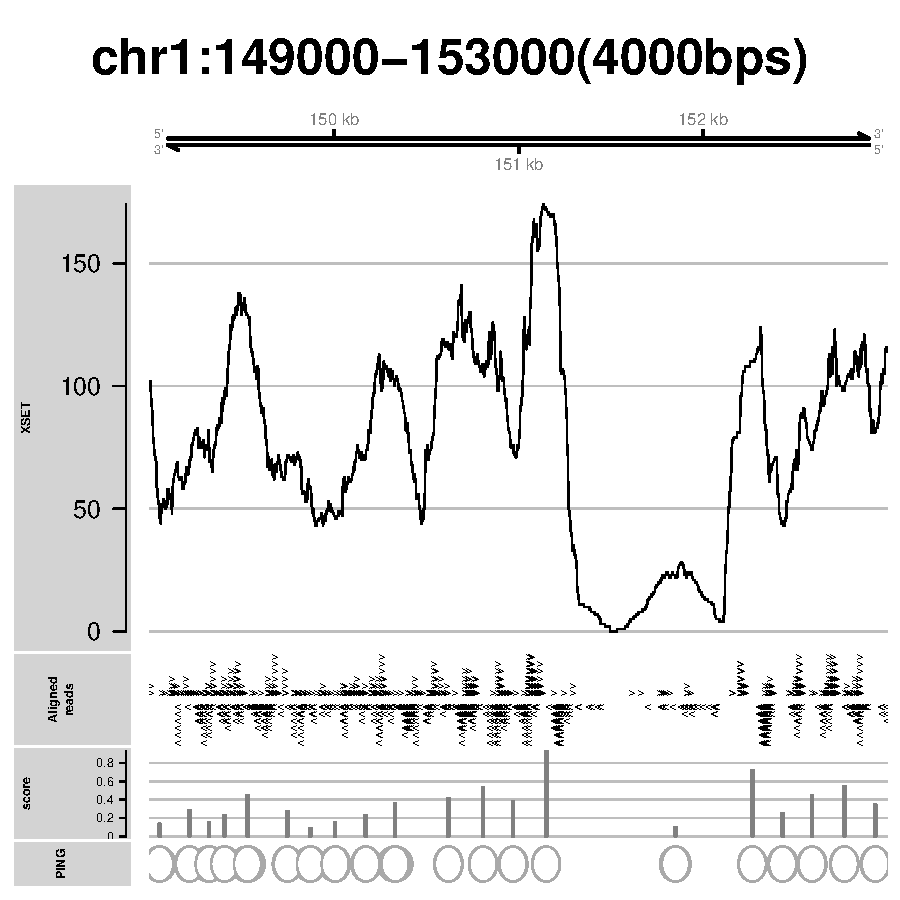
\includegraphics{PING-plotSummary}

The plot shows the coverage of the reads used as input, the start position of the forward and reverse reads and the predicted position of the nucleosome as well as the associated score for each nucleosome. The fuzzy gray border around some nucleosomes represents the uncertainty associated with its position.

This plotting function includes a filtering: by default, only nucleosomes having score over $0.05$ are shown. This can be modified by the users with the argument \texttt{scoreThreshold}. To hide the score track on the graph, the argument \texttt{scoreTrack} should be set to FALSE.

It is also possible to submit a list of several \texttt{postPING} results instead of a single \texttt{data.frame}. In this case, the graph shows nucleosome positioning tracks of the number of elelments in the list. For example, each track correponds to a different biological condition. 

\vspace{10pt}
Alternately, users experienced with \texttt{Gviz} can create their own desired plot by adding tracks produced by the following functions; a profie, aligned reads, and predicted nucleosome positions. Available track creation functions in the \texttt{PING} package are:

\begin{itemize}
\item \textbf{CoverageTrack}
\item \textbf{RawReadsTrack}
\item \textbf{NucleosomeTrack}
\end{itemize}

As an example, we first create $3$ tracks of a profile, aligned reads, and the predicted nucleosomes based on the data information and \texttt{postPING} result. In this new plot, we also want to screen out the nucleosomes with a score inferior to $0.1$:
\begin{Schunk}
\begin{Sinput}
> library(Gviz)
> cTrack <- CoverageTrack(ping, dataIP, "chr1", "gen")
> rTrack <- RawReadsTrack(ping, dataIP, "chr1", "gen", name = "Reads")
> nTrack <- NucleosomeTrack(PS, "chr1", "gen", scoreThreshold = 0.1, 
+     name = "NEW")
\end{Sinput}
\end{Schunk}

Then we add some information using track types issued from the \texttt{Gviz} package and finally use its plotting function: \texttt{plotTracks}.
\begin{Schunk}
\begin{Sinput}
> gTrack <- GenomeAxisTrack(add53 = TRUE, add35 = TRUE)
> aTrack <- AnnotationTrack(range = IRanges(start = 149500, end = 151000), 
+     showFeatureId = TRUE, id = "random annotation", col.title = "orange", 
+     chr = "chr1", gen = "gen", name = "custom")
> plotTracks(trackList = c(gTrack, cTrack, aTrack, rTrack, nTrack), 
+     main = "Custom plot", from = 149000, to = 153000)
\end{Sinput}
\end{Schunk}
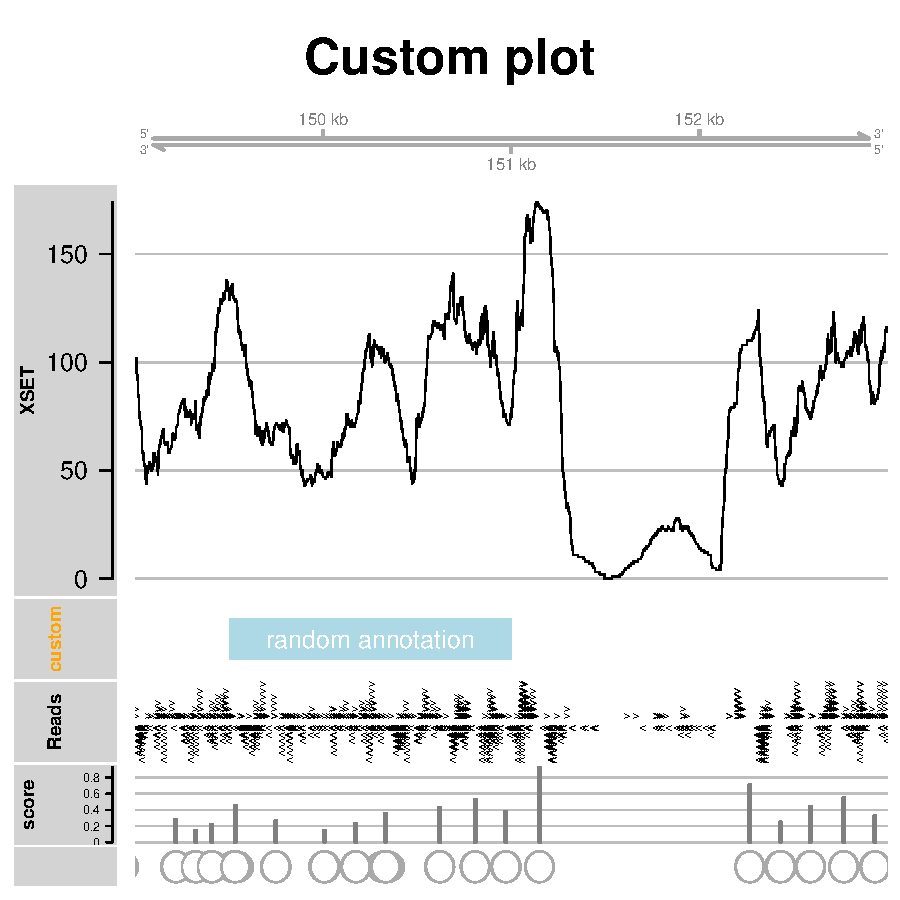
\includegraphics{PING-Gviz-tracks}

As expected, with the new filtering the nucleosomes of lower confidence score have been removed.

\end{document}
